\documentclass[12pt]{book}

\usepackage[dvips,letterpaper,margin=0.75in,bottom=0.5in]{geometry}
\usepackage{cite}
\usepackage{slashed}
\usepackage{graphicx}
\usepackage{amsmath}
\usepackage{braket}
\begin{document}

\newcommand{\ihbar}{\ensuremath{i \hbar}}
\newcommand{\Pss}{\ensuremath{\Psi^*}}
\newcommand{\dPsidt}{\ensuremath{ \frac{\partial \Psi}{\partial t} }}
\newcommand{\dPsidx}{\ensuremath{ \frac{\partial \Psi}{\partial x} }}
\newcommand{\ddPsidx}{\ensuremath{ \frac{\partial^2 \Psi}{\partial x^2} }}
\newcommand{\dPssdt}{\ensuremath{ \frac{\partial \Psi^*}{\partial t} }}
\newcommand{\dPssdx}{\ensuremath{ \frac{\partial \Psi^*}{\partial x} }}
\newcommand{\ddPssdx}{\ensuremath{ \frac{\partial^2 \Psi^*}{\partial x^2} }}

\title{PHY 115A \\ Lecture Notes:\\
The Wave Function \\ (Griffith's Chapter 1) \\}
\author{Michael Mulhearn}

\maketitle

\chapter{The Wave Function}

\section{The Experimental Foundation of Quantum Mechanics}

By the start of the 1900's classical physics had achieved a series of remarkable experimental and theoretical breakthroughs.
\begin{itemize}

\item Young's Double Slit experiment (1801) showed that when monochromatic light passes through a single slit followed by two double slits, the intensity of the light reaching a distant plane exhibits an interference pattern:
\begin{displaymath}
I(\theta) = I_0 \, \cos^2\left(\frac{\pi d}{\lambda} \sin \theta \right)
\end{displaymath}
where $\lambda$ is the wavelength of the light, $d$ the distance between the slit, $\theta$ the angle relative to the center of the slits, and $I_0$ the intensity at $\theta=0$.  

\item The Maxwell Equations (1861) unified the magnetic and electrical forces within a theory that accurately describes an array of phenomenon that is breathtaking in scope.  It predicted radio waves and how to produce and detect them.  It alluded to special relativity.  The theory showed that light was a propagating disturbance in the electromagnetic field: an EM wave.
\item JJ Thomson discovered the electron (1897) using cathode ray tubes and determined its charge to mass ratio.  The Millikan oil drop experiment (1909) determined the electron charge $e$.
\end{itemize}


\begin{figure}[thb]
\begin{center}
{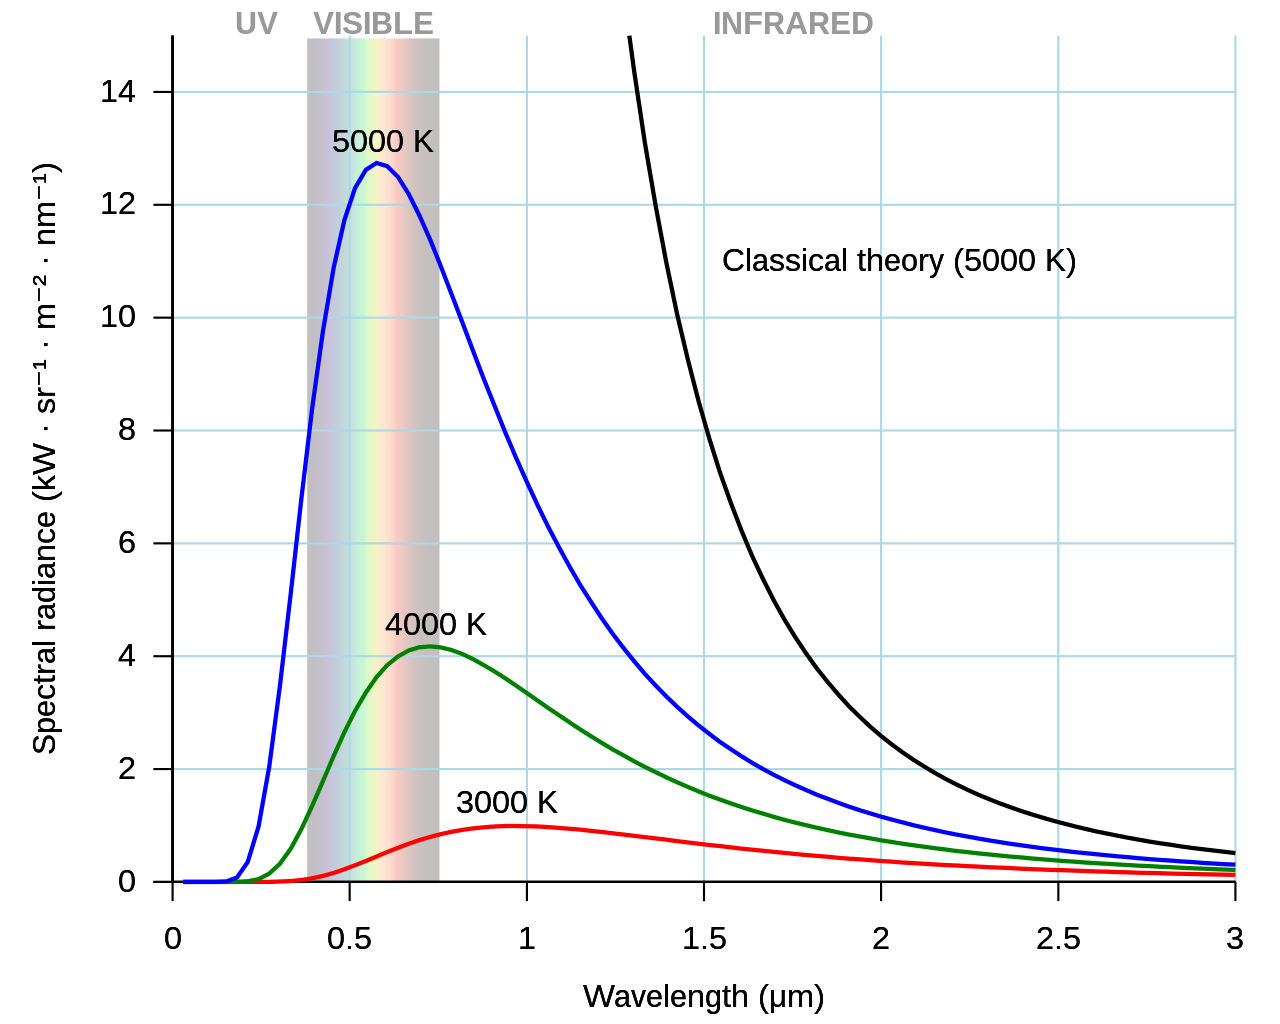
\includegraphics[width=0.40\textwidth]{figs/black_body.png}}
\end{center}
\caption{\label{fig:blackbody} The utraviolet catastrophe.}
\end{figure}


\noindent
Despite these impressive achievements, their were also shortcomings in the classical theory:
\begin{itemize}
\item The prediction of the classical theory for the spectral radiance of black body radiation failed spectacularly at low wavelength.  (See Fig.~\ref{fig:blackbody})
\item In the photoelectric effect, light shining on a material causes the emission of electrons.  The classical theory predicts that the kinetic energy of the photoelectrons emitted depends on the intensity of the light, but experiments showed it depended on the wavelength.  Below a certain wavelength for each material, there was no emission at all.
\item Atomic spectroscopy: hydrogen (and other atoms) were shown to emit electromagnetic radiation at specific wavelengths.  For the hydrogen atom, the quantized wavelengths are described by the empirically-determined Rydberg formula:
\begin{displaymath}
\frac{1}{\lambda} = R_H \left( \frac{1}{n_1^2} - \frac{1}{n_2^2} \right)
\end{displaymath}
where $1/R_H = 91~\rm nm$ and $n_1 < n_2$ are both quantum numbers.
\end{itemize}
The explanation for these phenomenon relied upon quantization: 
\begin{itemize}
\item Planck's Law: the observed spectral radiance from black body radiation can be accurately predicted if light consists of discrete quanta, called photons, with energy 
$$E = h \nu.$$  
The ultra-violet catastrophe is avoided because it requires a relatively large amount of energy to produce each ultra-violet photon.   
\item The surprising features of the photoelectric effect can also be understood as due to photons.  Individual photons below a certain wavelength do not have enough energy to liberate an electron, and the kinetic energy of the electrons depends on the energy of the photon, which depends on the wavelength of light, not the intensity. 
\item The Bohr model of the atom constrained electrons to orbits at discrete energy levels with angular momentum that is an integer ratio of Planck's constant.  This model perfectly predicted the Rydberg formula.
\end{itemize}

\noindent
As photons are massless, they have energy $E = pc$ where $p$ is there momentum, and so combining this with the Planck's Law:
\begin{eqnarray*}
E &=& p\,c = h \nu \\
\frac{c}{\nu} &=& \lambda = \frac{h}{p}\\
\end{eqnarray*}
where $\lambda$ is the wavelength of the light.  The quantization of photons inspired Louis de Broglie to make the brash and utterly correct hypothesis that matter behaves like a wave with wavelength
$$ \lambda = \frac{h}{p}.$$
This hypothesis was the beginning of our modern formulation of quantum mechanics.  Modern demonstrations of electron interference, as shown in Fig.~\ref{fig:elecint}, clearly reveal the wave nature of matter.

\begin{figure}[thb]
\begin{center}
{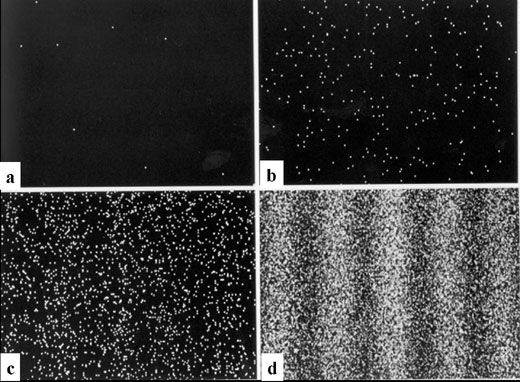
\includegraphics[width=0.40\textwidth]{figs/electron_interference.jpg}}
\end{center}
\caption{\label{fig:elecint} After passing through a double slit apparatus, the location of individual electrons are observed as dots of light.  When enough electrons are observed an interference pattern emerges.}
\end{figure}

The fascinating conversation between theory and experiment that led to the formulation of quantum mechanics is worthy of studying.  However, it isn't the easiest ways to come to terms with the shocking theory.  Instead of developing the theory piece by piece, we'll jump right to the Schr\"odinger Equation as our starting assumption, and work through the consequences.

\section{An Experimental Perspective}

\begin{itemize}

\item Never forget that physics is an {\bf experimental discipline}: the most compelling mathematical argument you can imagine could be rendered invalid by a single well-executed experiment.  

\item {\bf You cannot derive Quantum Mechanics.}  Quantum Mechanics is a set
of starting assumptions the consequences of which are consistent with experimental results.
It offers no explanation for the starting assumptions.

\item {\bf Derivations are useful for predicting the outcomes of future
experiments} based on the results from our previous experiments, within
the context of a theory.  The more successful we are at playing this little
game, the more confidence we have in the theory.

\item By this metric, {\bf Quantum Mechanics is an exceptionally successful theory!}

\item {\bf The starting assumptions are not unique.} You can learn
a lot by seeing how different assumptions lead to the same physical
theory.  We'll do some of this.

\end{itemize}

\section{The Schr\"odinger Equation}

Here's a summary of Griffiths sections 1.1-1.2.

\begin{itemize}

\item A state of a particle is described by its wave function $\Psi(x,t)$.

\item The wave function $\Psi(x,t)$ is a solution to the Schr\"odinger Equation (SE):
\begin{equation}
\label{eqn:se}
\ihbar \dPsidt = - \frac{\hbar^2}{2 m}\ddPsidx + V \Psi
\end{equation}
where $m$ is the mass of the particle, $V$ the potential energy function or just ``potential'', and:  

\item The reduced plank's constant $\hbar = \frac{h}{2 \pi} = 1.054573 \times 10^-34~\rm Js$.

\item The physical interpretation of the wave function is statistical.  The probability $P_{ab}(t)$ that the particle will be found between points $a$ and $b$ at time $t$ is:
\begin{equation}
\label{eqn:prob}
P_{ab}(t) = \int_a^b |\Psi(x,t)|^2 dx
\end{equation}
\end{itemize}

Suppose we divide the $x$-axis into six regions $A,B,C,D,E,F$ and the particle is in a state where it has equal probability to be found in any region at $t=0$.  At $t=0$ we observe the particle in region $C$.  Where was the particle before this measurement?  There are several schools of thought:
\begin{itemize}
\item realist:  The particle was already in region $C$ and we just didn't know that yet.
\item orthodox:  The particle wasn't in any one region, it was the measurement itself that caused one of several possible outcomes.
\item agnostic:  I don't know.  It doesn't matter where the particle was before a measurement, because physics is about predicting the outcome of measurements.
\end{itemize}
As we'll see later, John Bell showed that this seemingly philosophical question could be explored experimentally.  Of these three possibilities, the orthodox interpretation is the most supported by the experimental evidence.

\section{Review of Statistics and Probability}

Given that the physical interpretation of Quantum Mechanics is statistical, we'll review the relevant concepts from statistics. This is also covered in Griffiths sections 1.3.  

We refer to the outcome of a random process as a random variable.  Random variables can be discrete (countable): heads or tails from a coin flip, the number of children the next person you meet has had, the number of nuclear decays of a radioactive sample within a specified time interval.  Or random variables can be continuous:  the mass of fish that you have caught, the amount of time you must wait for the next bus to arrive, or the speed of the next bike that passes you.  Here we'll use variable $m$ for a discrete random variables that take on a countable number of distinct values $m=0,1.2,3,\ldots$.  We'll use $x$ to describe a continuous random variable $x$ on the interval $[-\infty, \infty]$. 

\subsection{Discrete and Continuous Random Variables}

In the discrete case, the probability of each outcome $m$ defines the probability distribution function $P(m)$.  To calculate the probability $P_{AB}$ that an outcome $m$ is any integer from $A$ to $B$ we need only sum the probability distribution function for those integers:
\begin{displaymath}
P_{AB} = \sum_{m=A}^{B} P(m).
\end{displaymath}
Because the probability of the outcome being any possible value is 1, we have the normalization condition:
\begin{displaymath}
\sum_{m=0}^{\infty} P(m) = 1
\end{displaymath}

In the case of a continuous random variable $x$, it is nonsensical to speak of the probability of any particular value of $x$.  Instead the probability of $x$ occurring within an interval $a < x < b$:
\begin{displaymath}
P_{ab} = \int_{a}^{b} \rho(x) \, dx
\end{displaymath}
The value of the probability distribution function $\rho(x)$ is not a probability, but instead a probability density, which we integrate to find the probability.  As the outcome must be some value of $x$ between $-\infty$ and $+\infty$ the normalization is:
\begin{displaymath}
\int_{-\infty}^{+\infty} \rho(x) \, dx = 1
\end{displaymath}
The probability distribution function of a continuous random variable is called a probability density function (PDF).  A discrete probability distribution is sometimes referred to
as probability mass function (PMF), to draw upon an analogy with physical mass and density: a PDF is probability per unit volume (1-D volume in this case) while
a PMF is simply a probability.

\subsection{Mean and Variance}

Given a probability distribution our most urgent questions are generally ``what is a
typical outcome?'' and ``how widely will outcomes typically vary from
one another?''.  There are a number of ways to give a quantitative answer to the first question,
but generally the most useful answer is the mean value of the
distribution, $\mu$, which we calculate as a weighted average across
all possible outcomes.  For a discrete random variable we calculate a sum:
\begin{equation}
\label{eqn:mudis}
\mu = \sum_{m=0}^{\infty} m \, P(m)
\end{equation}
For a continuous probability distribution we integrate instead:
\begin{equation}
\mu = \int_{-\infty}^{+\infty} x \, \rho(x) \, dx 
\end{equation}
across a range appropriate to the situation, typically $[-\infty,\infty]$.

The mean value is an example of an expectation value.  In general, the
expectation value of a function $f(x)$ of a random variable $x$ drawn
from a probability distribution function $P(x)$ is:
\begin{displaymath}
\braket{f(x)} \equiv \int_{-\infty}^{+\infty} f(x) \, \rho(x) \,dx.
\end{displaymath}
For a discrete random variable, the integral becomes a sum:
\begin{displaymath}
\braket{f(m)} \equiv \sum_m f(m) \, P(m) 
\end{displaymath}
Using this notation, we can define the mean as the expectation value of the random variable:
\begin{displaymath}
\mu \equiv \braket{x}
\end{displaymath}

To answer the second question, we define an expectation value
which characterizes the variation of outcomes from the mean value,
which we call the variance ($\sigma^2$) of the distribution:
\begin{displaymath}
\sigma^2 \equiv \braket{(x-\mu)^2}.
\end{displaymath}
The square root of the variance is referred to as the
standard deviation ($\sigma$).

There are other ways to quantify the variation from outcome to
outcome, but they are generally inferior to the variance in some way.
For example $\braket{x-\mu}$ can be zero, even for wide distributions,
as long as $P(x)$ is symmetric.  The quantity $\braket{|x-\mu|}$
(called the average deviation) avoids this pitfall but is generally
much harder to calculate, due to the absolute value.

The variance, on the other hand, is quite convenient to calculate.
For example, you can show that:
\begin{equation}
\label{eqn:varhw}
\braket{(x-\mu)^2} = \braket{x^2} -\braket{x}^2.
\end{equation}
We need only calculate $\braket{x}$ and $\braket{x^2}$ in order
to determine both the mean and variance of a distribution.

\section{Normalization of the Wave Function}

This material is covered in Griffiths section 1.4.  
\begin{itemize}
 \item If $\Psi(x,t)$ is a solution to the SE, then so is $k \cdot \Psi(x,t)$ for any value $k$ (check!)  So it would seem we could make the probability density $|\Psi(x,t)|^2$ any value that we like and still satisfy the SE!  
 \item In fact, we are constrained in our choice by the realization that the probability of finding the particle {\em somewhere} must be 1, and so we must choose the normalization of $\Psi$ such that:
\begin{equation}
\label{eqn:norm}
\int_{-\infty}^{+\infty} |\Psi(x,t)|^2 dx = 1
\end{equation}

\item If $\Psi(x,t)=0$ for all $x$ we cannot normalize $\Psi$.
 \item If the integral:
$$\int_{-\infty}^{+\infty} |\Psi(x,t)|^2 dx$$
diverges then we cannot normalize $\Psi$.
\item Being good physicists, we simply throw away useless unphysical solutions that cannot be normalized, and we are never troubled by them again! 
\end{itemize}

But now here's a troubling throught.  Suppose at $t=0$, we have normalized $\Psi(x,t)$ such that
$$\int_{-\infty}^{+\infty} |\Psi(x,0)|^2 dx = 1$$.  
From this point on, the time dependence of $\Psi(x,t)$ is given by the SE, outside of our control.  What if changes in such a way that:
$$\int_{-\infty}^{+\infty} |\Psi(x,t)|^2 dx \neq 1$$ 
at later times?  Might we have to renormalize $\Psi(x,t)$ again at each $t$?  What would we make of $d\Psi/dt$ in this case?

Fortunately, solutions to the SE preserve their normalization.  We can show this using the SE.  We note that:
$$\frac{d}{dt}\int_{-\infty}^{+\infty} |\Psi(x,t)|^2 \, dx  = 
\int_{-\infty}^{+\infty} \frac{\partial}{\partial t} |\Psi(x,t)|^2\, dx.$$ 
Working on the integral:
\begin{eqnarray*}
\frac{\partial}{\partial t} |\Psi(x,t)|^2 &=&  \frac{\partial}{\partial t} (\Psi^* \Psi) \\[7pt]
  &=&  \frac{\partial \Psi^*}{\partial t} \Psi + \Psi^* \frac{\partial \Psi}{\partial t} \\
\end{eqnarray*}
Reworking SE:
\begin{eqnarray*}
\label{eqn:se}
\ihbar \dPsidt &=& -  \frac{\hbar^2}{2 m}\,\ddPsidx + V \Psi \\[7pt] 
       \dPsidt &=& \;\; \frac{\ihbar}{2 m}\,\ddPsidx - \frac{i V}{\hbar} \Psi \\[7pt]
       \dPssdt &=& - \frac{\ihbar}{2 m}\,\ddPssdx + \frac{i V}{\hbar} \Psi^* \\[7pt]
\end{eqnarray*}
where in the last step we've taken the complex conjugate of the preceding equation.  Substituting these results we have:
\begin{eqnarray}
\frac{\partial}{\partial t} |\Psi(x,t)|^2 &=&  \frac{\ihbar}{2 m} 
\left( \Psi^* \ddPsidx - \ddPssdx \Psi\right) \notag \\[7pt]
\label{eqn:dtpp}
  &=& \frac{\ihbar}{2 m} \;
\frac{\partial}{\partial x} \, \left( \Psi^* \dPsidx - \dPssdx \Psi\right)
\end{eqnarray}
So now:
\begin{eqnarray*}
\frac{d}{dt}\int_{-\infty}^{+\infty} |\Psi(x,t)|^2 \, dx  &=& 
\frac{\ihbar}{2 m} \, \int_{-\infty}^{+\infty}  \frac{\partial}{\partial x} \, \left( \Psi^* \dPsidx - \dPssdx \Psi\right) dx\\[7pt]
&=&  \frac{\ihbar}{2 m} \, \left. \left( \Psi^* \dPsidx - \dPssdx \Psi\right) 
\right\rvert_{-\infty}^{+\infty}\\[7pt]
&=& 0
\end{eqnarray*}
where in the last step we've used the fact that the wave function and it's derivative must go to zero at infinity to be physical.

\section{Review of Integration by Parts}

We'll make use of integration by parts in the following sections, so let's review the idea.  We apply the chain rule to the functions $u(x)$ and $v(x)$:
$$\frac{d(uv)}{dx} = u\frac{dv}{dx} + v\frac{du}{dx}$$
and then integrate both sides:
$$\int_a^b\frac{d(uv)}{dx} \, dx = \int_a^b u \frac{dv}{dx} \, dx + \int_a^bv\frac{du}{dx} \, dx$$
By the fundamental theorem of calculus:
$$\int_a^b\frac{d(uv)}{dx} = \left. uv \right\rvert_{a}^{b}$$
If the product $u(x)\,v(x)$ vanishes at $x = a$ and $x = b$ then
$$\left.uv \right\rvert_{a}^{b} = 0$$
and so:
\begin{equation}
\label{eqn:intparts}
\int_{a}^{b} u \frac{dv}{dx} \, dx =  - \int_{a}^{b} v \frac{du}{dx} \, dx
\end{equation}
Suppose a definite integral consists of two parts, one of which ($dv/dx$ here) is a derivative with respect to the integration variable ($x$ here).  Further suppose that the integrand with the derivative removed ($uv$ here) vanishes at the limits of the integration.  In this case, we can move the differentiation between parts of the integrand (from $v$ to $u$ here) by adding a negative sign.

\section{Position and Momentum Operators}
\begin{itemize}
\item  From the probability interpretation of the wave function $\rho(x) = | \Psi | ^2$, we define the expectation value of the $x$ position as:
$$\braket{x} \equiv \int_{-\infty}^{+\infty} x \, \rho(x) \,dx = \int_{-\infty}^{+\infty} x \, |\Psi|^2 \,dx$$
\item There is some subtlety here: the expectation value for the observable $x$ is the mean value of the results of many repeated measurements of the $x$ position of a particle {\em always starting} in the same state $\Psi$.  
\item Due to the collapse of the wave function, repeated measurements of the $x$ position of the same particle {\em after} it was already observed at some position $x=a$ would reproduce the same result (to within the experiments ability to do so before the particle's state changes).
\end{itemize}

In classical physics, the state of a particle is completely determined from it's position and momentum.  So it is natural to consider the expectation value for the momentum: 
\begin{eqnarray*}
\braket{p} &=& m \frac{d}{dt} \braket{x} \\[7pt] 
&=& m \int_{-\infty}^{+\infty} x \, \frac{\partial}{\partial t} |\Psi|^2 \,dx \\[7pt]
\end{eqnarray*}
We already worked out the time derivative in the integrand before (Equation~\ref{eqn:dtpp}) so we have:
\begin{eqnarray*}
\braket{p} &=&  \frac{\ihbar}{2} \int_{-\infty}^{+\infty} x \, \frac{\partial}{\partial x} \, \left( \Psi^* \dPsidx - \dPssdx \Psi\right) \,dx \\[7pt]
\end{eqnarray*}
We can use integration by parts to move the outer partial derivative onto the $x$:
\begin{eqnarray*}
\braket{p} &=&  -\frac{\ihbar}{2} \int_{-\infty}^{+\infty} \frac{\partial x}{\partial x} \, \left( \Psi^* \dPsidx - \dPssdx \Psi\right) \,dx \\[7pt]
&=&  -\frac{\ihbar}{2} \int_{-\infty}^{+\infty} \, \left( \Psi^* \dPsidx - \dPssdx \Psi\right) \,dx \\[7pt]
\end{eqnarray*}
And one more application of integration by parts to second term in the parenthesis:
\begin{eqnarray}
\braket{p} &=&  -\ihbar \, \int_{-\infty}^{+\infty} \, \left( \Psi^* \dPsidx \right) \,dx \notag \\[7pt]
 &=& \int_{-\infty}^{+\infty} \, \Psi^* \left[ -\ihbar \frac{\partial}{\partial x}\right] \Psi \,dx 
\label{eqn:derivpop} \end{eqnarray}
Compare to the expectation value for the position:
\begin{eqnarray}
\braket{x} 
 &=& \int_{-\infty}^{+\infty} \, \Psi^* \left[ x \right] \Psi \,dx 
\end{eqnarray}

In general, we calculate expectation value of an observable $o$
using the corresponding {\em operator} $\hat{o}$:
\begin{eqnarray}
\braket{o}  &=& \int_{-\infty}^{+\infty} \, \Psi^* \left[ \hat{o} \right] \Psi \,dx 
\end{eqnarray}
For the position observable we have the position operator 
\begin{equation}
\hat{x} = x.
\end{equation}
For the momentum observable with have the momentum operator 
\begin{equation}
\hat{p} = - \ihbar \frac{\partial}{\partial x}.
\end{equation}
We can construct the operator $\hat{f}$ for any classical function of position and momentum $f(x,p)$ by substituting $\hat{p}$ and $\hat{x}$ for $p$ and $x$.
\begin{eqnarray}
\braket{f(x,p)}  &=& \int_{-\infty}^{+\infty} \, \Psi^* \left[ f(\hat{x},\hat{p}) \right] \Psi \,dx 
\end{eqnarray}
Since the position and momentum completely define the state of a classical particle, any dynamical variable can be calculated from x and p.  Therefore, this is a prescription for calculating the expectation value of any classical dynamical variable.

Have a close look at Equation~\ref{eqn:derivpop}.  Had we applied integration by parts to the first term instead of the section, we would have instead concluded:
\begin{eqnarray*}
\braket{p} &=&  
\int_{-\infty}^{+\infty} \, \left(\left[ \ihbar \frac{\partial}{\partial x}\right] \Psi^* \right) \Psi\,dx \\
&=& \int_{-\infty}^{+\infty} \, \left(\left[ -\ihbar \frac{\partial}{\partial x}\right] \Psi \right)^* \Psi\,dx \\
&=& \int_{-\infty}^{+\infty} \, \left( \hat{p} \Psi \right)^* \Psi\,dx 
\end{eqnarray*}
so we would have identified the same momentum operator, but operating on $\Psi^*$.  We'll return to this later.

\section{Ehrenfest's Theorem}
\begin{eqnarray*}
\frac{d \braket{p}}{dt} &=& \frac{d}{dt} \int_{-\infty}^{+\infty} \, \Psi^* \, \hat{p} \, \Psi \,dx \\[7pt]
&=& -\ihbar \int_{-\infty}^{+\infty} \, \frac{\partial}{\partial t} \left(\Psi^* \dPsidx\right) \,dx \\[7pt]
&=& -\ihbar \int_{-\infty}^{+\infty} \, \left( \dPssdt \dPsidx + 
\Psi^* \frac{\partial}{\partial x} \dPsidt \right) \,dx \\[7pt]
\end{eqnarray*}
where in the last part we have used:
$$\frac{\partial}{\partial t} \dPsidx = \frac{\partial}{\partial x} \dPsidt$$
now using integration by parts on the second term:
\begin{eqnarray*}
\frac{d \braket{p}}{dt} &=& -\ihbar \int_{-\infty}^{+\infty} \, 
\left( \dPssdt \dPsidx - \dPssdx \dPsidt \right) \,dx \\[7pt]
&=& -\ihbar \int_{-\infty}^{+\infty} \, 
\left( \left[ -\frac{\ihbar}{2 m}\,\ddPssdx + \frac{i V}{\hbar} \Pss \right] \dPsidx 
- \dPssdx \left[ \frac{\ihbar}{2 m}\,\ddPsidx - \frac{i V}{\hbar} \Psi \right] \right) \,dx \\[7pt]
&=& -\frac{\hbar^2}{2 m} \int_{-\infty}^{+\infty} \, \left(\ddPssdx \dPsidx + \dPssdx \ddPsidx\right)
+ \int_{-\infty}^{+\infty} V \left( \Pss \dPsidx + \dPssdx \Psi \right) \, dx \\[7pt]
&=& -\frac{\hbar^2}{2 m} \int_{-\infty}^{+\infty} \, \frac{\partial}{\partial x} \left(\dPssdx \dPsidx\right) dx
+ \int_{-\infty}^{+\infty} V \frac{\partial}{\partial x} \left( \Pss \Psi \right) \, dx \\[7pt]
\end{eqnarray*}
The first integral vanishes\footnote{If you want to go for the hat trick (three scores in one game) on using integration by parts, you can do it here, noting that $d1/dx = 0$.} and using integration by parts on the second integrand:
\begin{eqnarray*}
\frac{d \braket{p}}{dt} &=& -\int_{-\infty}^{+\infty} \frac{\partial V}{\partial x} \Pss \Psi \, dx \\[7pt]
\end{eqnarray*}
so now:
\begin{eqnarray}
\label{eqn:ehrenfest}
\frac{d \braket{p}}{dt} &=& - \braket{\frac{\partial V}{\partial x}}
\end{eqnarray}
which is known as Ehrenfest's Theorem.

Newton's Law in one dimension in classical physics can be written as:
\begin{eqnarray}
\label{eqn:ehrenfest}
\frac{dp}{dt} &=& -\frac{dV}{dx}
\end{eqnarray}

which remains true in Quantum Mechanics in an average sense.

\section{The Uncertainty Principle}

We can generalize the variance described in the review of statistics to any observable $o$, and note that the variance $\sigma^2_o$ of an observable $o$ can be calculated as:
\begin{displaymath}
\sigma_o^2 \equiv \braket{\,(o-\braket{o})^2\,} = \braket{o^2}-\braket{o}^2
\end{displaymath}
The square root of the variance is referred to as the uncertainty.  So $\sigma_o$ is the uncertainty in $o$.

The variance of the position $x$ is:
\begin{displaymath}
\sigma_x^2 \equiv \braket{\,(x-\braket{x})^2\,} = \braket{x^2}-\braket{x}^2
\end{displaymath}
where:
\begin{eqnarray}
\braket{x} 
 &=& \int_{-\infty}^{+\infty} \, \Psi^* \left[ \hat{x} \right] \Psi \,dx \\
 &=& \int_{-\infty}^{+\infty} \, x|\Psi|^2 \,dx 
\end{eqnarray}
and
\begin{eqnarray}
\braket{x^2} 
 &=& \int_{-\infty}^{+\infty} \, \Psi^* \left[ \hat{x}^2 \right] \Psi \,dx \\
 &=& \int_{-\infty}^{+\infty} \, x^2|\Psi|^2 \,dx 
\end{eqnarray}
The variance of momentum $p$ is:
\begin{displaymath}
\sigma_p^2 \equiv \braket{\,(p-\braket{p})^2\,} = \braket{p^2}-\braket{p}^2
\end{displaymath}
where:
\begin{eqnarray}
\braket{x} 
 &=& \int_{-\infty}^{+\infty} \, \Psi^* \left[ \hat{p} \right] \Psi \,dx \\[8pt]
 &=& -\ihbar \int_{-\infty}^{+\infty} \, \Psi^* \; \dPsidx \; dx \\
\end{eqnarray}
and
\begin{eqnarray}
\braket{x^2} 
 &=& \int_{-\infty}^{+\infty} \, \Psi^* \left[ \hat{p}^2 \right] \Psi \,dx \\[8pt]
 &=& -\hbar^2 \int_{-\infty}^{+\infty} \, \Psi^* \; \ddPsidx \; dx \\
\end{eqnarray}

The Heisenberg uncertainty principle states that:
\begin{equation}
\sigma_x \sigma_p \, \geq \, \frac{\hbar}{2}
\end{equation}

This is easily the most famous result of quantum mechanics.  But we aren't ready to prove it yet. We will come back to that once we are better equipped to do so.

Griffiths section 1.6 gives a good intuitive explanation that goes like this:
\begin{itemize}
\item The de Broglie hypothesis relates a particles momentum to it's wavelength:
\begin{equation}
p = \frac{h}{\lambda}
\end{equation}
(we aren't equipped yet to proof this yet either)
\item Waves that have a well defined wavelength (e.g. an entire sine wave) do not have a well defined position.
\item Waves that have a well defined position (e.g. a localized splash) do not have a well defined wavelength.
\end{itemize}

Don't worry if this doesn't seem clear yet.  We'll but this on very firm ground later!

\section{Chapter Review}

We are considering a particle of mass $m$, in one dimension $x$, in a potential $V$.

\begin{itemize}
\item The state of a particle is described by its wave function $\Psi(x,t)$.
\item The wave function $\Psi(x,t)$ is a solution to the Schr\"odinger Equation (SE):
\begin{equation}
\label{eqn:se}
\ihbar \dPsidt = - \frac{\hbar^2}{2 m}\ddPsidx + V \Psi
\end{equation}
\item The physical interpretation of the wave function is statistical.  The probability $P_{ab}(t)$ that the particle will be found between points $a$ and $b$ at time $t$ is:
\begin{equation}
\label{eqn:prob}
P_{ab}(t) = \int_a^b |\Psi(x,t)|^2 dx
\end{equation}
\item The wave functions are normalized such that
\begin{equation}
\int_{-\infty}^{+\infty} |\Psi(x,t)|^2 dx = 1
\end{equation}
\item Once a wave function is normalized, it will remain normalized for all time as a consequence of the Schr\"odinger equation.
\item Measurements of observable quantities are associated with operators.  Given an operator $\hat{o}$ we can calculate the expectation value for the observable $o$ as:
\begin{eqnarray}
\braket{o}  &=& \int_{-\infty}^{+\infty} \, \Psi^* \left[ \hat{o} \right] \Psi \,dx 
\end{eqnarray}
The operator acts toward its right.
\item For the position observable we have the position operator 
\begin{equation}
\hat{x} = x.
\end{equation}
\item For the momentum observable we have the momentum operator 
\begin{equation}
\hat{p} = - \ihbar \frac{\partial}{\partial x}.
\end{equation}
\item Any classical dynamical variable can be calculated from the position and momentum, and we can calculate its expectation value as:
\begin{eqnarray}
\braket{f(x,p)}  &=& \int_{-\infty}^{+\infty} \, \Psi^* \left[ f(\hat{x},\hat{p}) \right] \Psi \,dx 
\end{eqnarray}
\item Newtons law is still true, but only in an average sense, by Ehrenfest's Theorem:
\begin{eqnarray}
\frac{d \braket{p}}{dt} &=& - \braket{\frac{\partial V}{\partial x}}
\end{eqnarray}
\item The variance $\sigma^2_o$ of an observable $o$ can be calculated as:
\begin{equation}
\sigma_o^2 \equiv \braket{\,(o-\braket{o})^2\,} = \braket{o^2}-\braket{o}^2
\end{equation}
The square root of the variance is referred to as the uncertainty.  
\item The Heisenberg uncertainty relation states that:
\begin{equation}
\sigma_x \sigma_p \, \geq \, \frac{\hbar}{2}
\end{equation}

\end{itemize}

\end{document}




